\documentclass[12pt]{amsart}

\usepackage{fullpage,hyperref,url}
\usepackage[pdftex]{graphicx}

\title{Project Proposal: Quintic Spectrahedra}
\author{Jacob Emmert-Aronson}
\author{Moor Xu}
\date{March 12, 2014}
\begin{document} 
\maketitle

\emph{Spectrahedra} of degree $n$ in $\mathbb{R}^k$ are convex bodies
given by $k$-dimensional affine slices of the cone of $n \times n$
positive semidefinite matrices.  They arise as feasible domains in
semidefinite programming and each is described by a linear matrix
inequality.
\vspace\baselineskip

\begin{center}

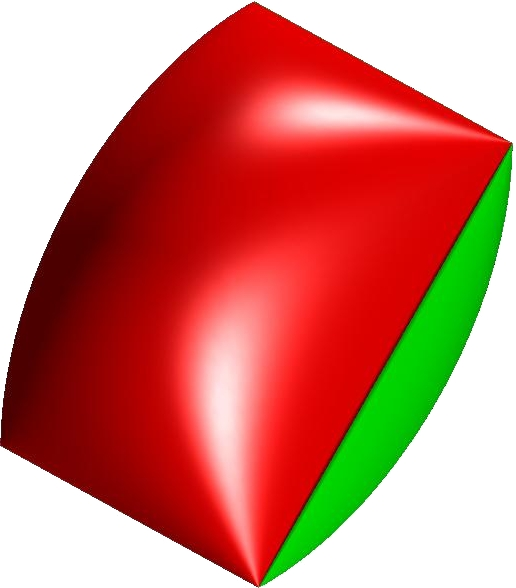
\includegraphics[scale=.15]{pillow.jpg}
\vspace\baselineskip

{\small
\emph{The pillow}: the spectrahedron
$
\begin{pmatrix}
  1&x&0&x\\
  x&1&y&0\\
  0&y&1&z\\
  x&0&z&1
\end{pmatrix}
\succeq 0\text.$  Here $k=3,\, n=4$.}
\end{center}
\vspace\baselineskip

Because the cost function of an SDP is linear, the optimal point
always lies on the surface.  One interesting and practically useful
question is the likelihood for the result of an optimization to be a
node, one of the corner points seen when visualizing the
spectrahedron.  A generic matrix represented by a point on the surface
of the spectrahedron has rank $n-1$, while the matrix at a node
typically has rank $n-2$.  This low-rank property of nodes often
translates to easier computation.

We propose to study the nodal structure of quintic spectrahedra in
$\mathbb{R}^3$.  We wish to study the possible numbers of nodes on the
surface of a spectrahedron as well as real nodes on the symmetroid,
its Zariski closure.  We will also evaluate the effect of these
quantities on the probability that a random optimization problem will
select a node.

To carry this out, we will generate random spectrahedra and compute
the positions of nodes, while also running multiple optimization
problems on each.  Much of the code for this is already
written.  Currently, singular is used to determine locations of nodes
through a Gr\"obner basis algorithm; due to apparent numeric
instabilities, however, this misidentifies nodes in certain edge
cases.  We hope to replace this with the homotopy algorithms
implemented in bertini, which produce more reliable results.

We also plan to learn what has been done in the case of quartic spectrahedra,
and see if any of that theory generalizes to the quintic case.


%%%%%%%%%%%%%%%%%%%%%%%
\bibliographystyle{amsplain}
\bibliography{references}
\nocite{*}

\end{document} 


